\chapter{Introducción}

En este capítulo exponemos el problema que buscamos resolver y mencionamos brevemente los acercamientos más populares.

\section{Identificación del problema}
Es común encontrar datos de series de tiempo cuya organización refleja una estructura de jerarquía. Cualquier cadena u institución con presencia nacional o internacional debe considerar las delimitaciones geográficas en su planeación. Por ejemplo, la venta de un artículo se puede visualizar como su venta en una tienda específica, en un estado o en una región. Similarmente, dicho artículo puede ser parte de una categoría específica que a su vez es parte de una línea de producto, por lo que su venta debe estar reflejada en estos niveles. 

Una muestra de lo anterior se observa en la figura \ref{fig:jerarquia_1}. A este tipo de datos cuyo valor puede ser agregado y que refleja un orden temporal se le conoce como series de tiempo jerárquicas \cite{hyndman2018forecasting}.

Realizar predicciones para datos de series de tiempo es un problema bien conocido y con distintas técnicas y modelos según el caso al que nos enfrentemos. Nos interesan estas predicciones, pues ayudan en la toma de decisiones complejas ante mucha incertidumbre (por ejemplo, resulta complicado pronosticar la demanda futura de turistas en el próximo verano en una zona o la demanda de SKUs en las distintas tiendas de una cadena empresarial) \cite{abolghasemi2020model}.

En particular, las series de tiempo jerárquicas tienen la dificultad adicional de conciliar los pronósticos, esto es, de garantizar que la suma de las predicciones individuales es equivalente a realizar una predicción del total general (podemos pronosticar la demanda de turistas en un hotel en una región y así para todo el país. La suma de estas debe ser equivalente al pronóstico individual de la demanda de la temporada de verano completa). El proceso de conciliación típicamente degrada la exactitud del pronóstico \cite{hyndman2014optimally}.  

Para resolver lo anterior, se tienen las técnicas de ''abajo-arriba", ''arriba-abajo'' y ''punto medio'' donde usamos como punto pivote la predicción en algún nivel de la jerarquía. Dado que la conciliación se hace como un paso posterior al pronóstico, existen trabajos dedicados al relajamiento del cómputo requerido para pronosticar y conciliar en un mismo paso como el de \cite{ashouri2019fast}.

También está el acercamiento combinatorio que no se basa en un nodo pivote sino que utiliza toda la información de la jerarquía para conciliar las predicciones. La información es codificada con un sistema de pesos que dependen principalmente de la jerarquía y no los datos. Este acercamiento ha visto mucha actividad reciente, pues tecnologías y técnicas como las de Machine Learning (ML) intentan descifrar la mejor manera de presentar el sistema de pesos \cite{abolghasemi2020model, abolghasemi2019machine, spiliotis2020hierarchical}.

Este documento sigue la siguiente estructura: en el capítulo 2 analizamos el marco teórico para la predicción con series de tiempo jerárquicas; en el capítulo 3 exponemos un modelo que realiza predicciones con ayuda de ML y exhibimos los resultados obtenidos, y en el último capítulo, se indican nuestras conclusiones.

\begin{figure}
    \centering
    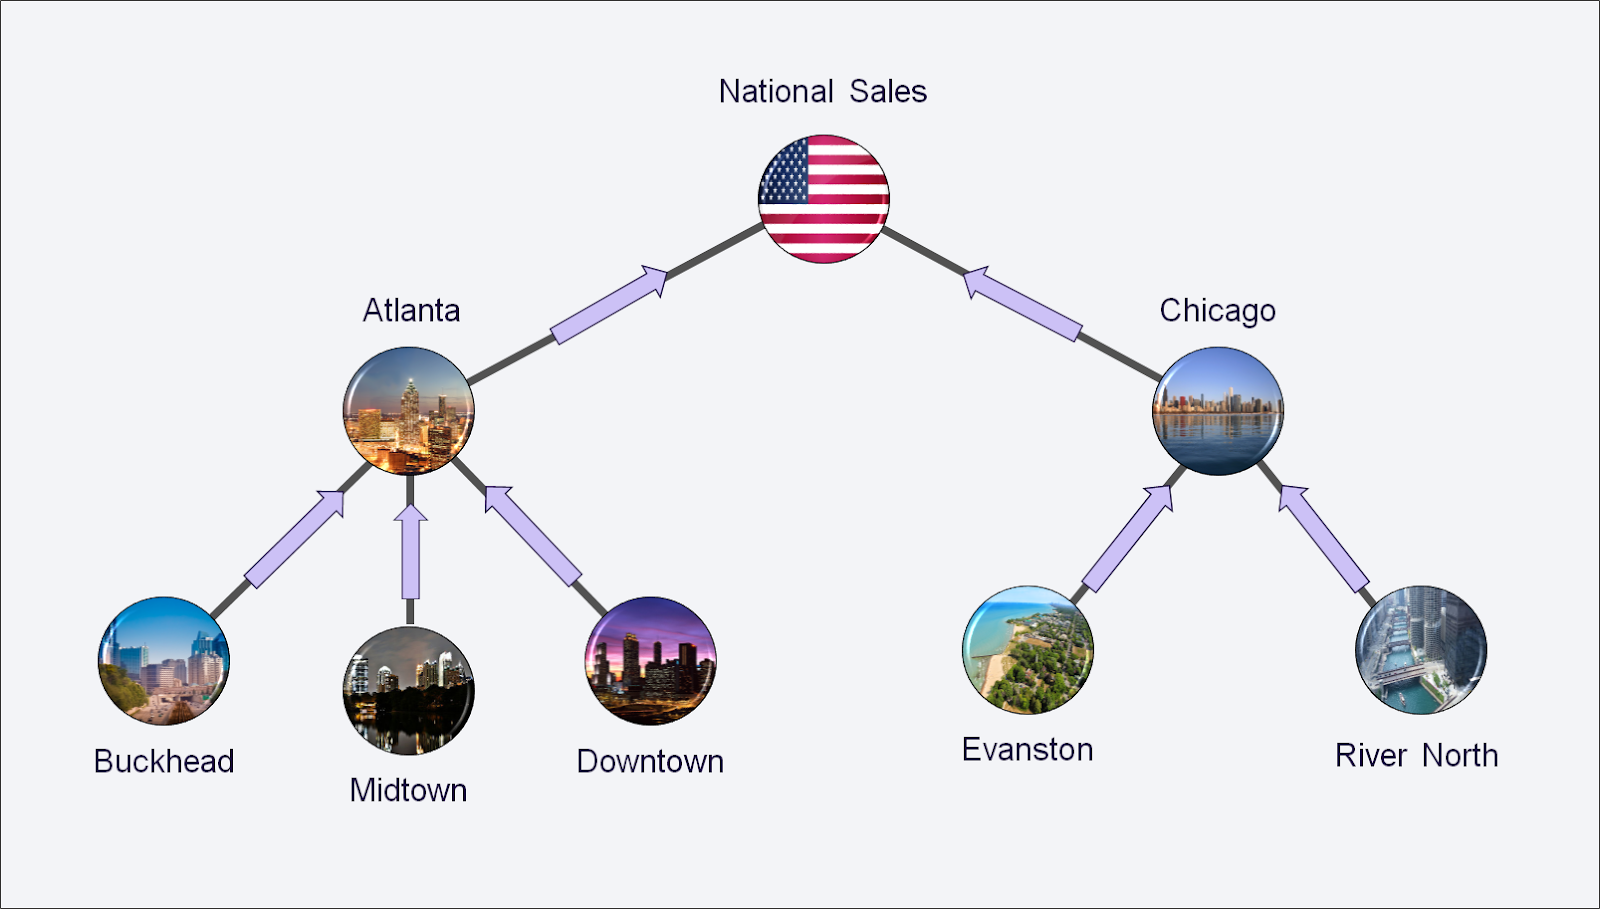
\includegraphics[width=0.9\textwidth]{imgs/jerar1.png}
    \caption{Ejemplo visual para las ventas nacionales de un producto con estructura de jerarquía}.
    \label{fig:jerarquia_1}
\end{figure}